% !TEX TS-program = XeLaTeX
\documentclass[a4paper]{article}


% https://tex.stackexchange.com/a/5365
% Must
\usepackage[table]{xcolor}

\usepackage{tabularx}


\usepackage{tikz}
\usepackage{fontspec,lipsum}
%\usepackage{color}


% https://tex.stackexchange.com/questions/172234/define-and-set-length-in-one-command
\newcommand{\deflen}[2]{%      
    \expandafter\newlength\csname #1\endcsname
    \expandafter\setlength\csname #1\endcsname{#2}%
}

\newcommand{\goldenratio}{1.618}

% Page margins
\deflen{horizontalmarg}{1.0cm}
\deflen{verticalmarg}{\dimexpr(\goldenratio\horizontalmarg)}

\usepackage[top=\the\verticalmarg, bottom=\the\verticalmarg, 
  left=\the\horizontalmarg, right=\the\horizontalmarg]{geometry}


\deflen{lowerbaroffset}{0.8cm}

\deflen{contentswidth}{\dimexpr(\paperwidth-2\horizontalmarg)}
\deflen{contentsheight}{\dimexpr(\paperheight-2.01\verticalmarg)}

\deflen{halfwidth}{\dimexpr(0.5\contentswidth)}


\deflen{paramarg}{0.5cm}

\deflen{colwidth}{\dimexpr(\halfwidth-\paramarg)}

\deflen{lowersectionstart}{\dimexpr(0.5\contentsheight)}
\deflen{headermarg}{2cm}

%% The vertical lines at which things should align
\deflen{haligni}{0cm}
\deflen{halignii}{\colwidth}
\deflen{haligniii}{\dimexpr(\halfwidth+\paramarg)}
\deflen{haligniv}{\dimexpr(\contentswidth)}


%% Horizontal lines at which things should align
\deflen{valigni}{\contentsheight}
\deflen{valignii}{\dimexpr(\contentsheight-\headermarg)}
\deflen{valigniii}{\lowersectionstart}
\deflen{valigniv}{\dimexpr(\lowersectionstart-\headermarg)}


% A paragraph: Args (X, Y, text)
\newcommand{\anemoparagraph}[3]{
  \node[anchor=north west,style={inner sep=0,outer sep=0}] at (#1,#2) {
    \begin{minipage}[l]{\the\colwidth}
      #3
    \end{minipage}
  };
}

% Draw a vertical bar across the contents area
\newcommand{\vhelper}[1]{\draw[color=gray] (#1,0cm) -- (#1,\the\contentsheight);}

% Draw a horizontal bar across the contents area
\newcommand{\hhelper}[1]{\draw[color=gray] (0cm,#1) -- (\the\contentswidth,#1);}

% Display helper lines
\newcommand{\helpers}{
  \draw[color=gray] (0,0) rectangle (\the\contentswidth, \the\contentsheight);
  \vhelper{\the\halignii}
  \vhelper{\the\haligniii}
  \hhelper{\the\valignii}
  \hhelper{\the\valigniii}
  \hhelper{\the\valigniv}
}

% A4: 21.0 × 29.7
\pagenumbering{gobble}
\setmainfont[Path=../fonts/]{Muli-Regular.ttf}

% (x, y, contents)
\newcommand{\mainheader}[3]{
  \setmainfont[Path=../fonts/]{BoingBold.otf}
  \node[anchor=north west] at (#1,#2) {\Huge #3};
  \setmainfont[Path=../fonts/]{Muli-Regular.ttf}
}



\definecolor{Anemored}{RGB}{255, 33, 63}


% https://tex.stackexchange.com/a/159576
\newcommand{\HRule}[1][\medskipamount]{\par
  \vspace*{\dimexpr-\parskip-\baselineskip+#1}
  \noindent\rule{\linewidth}{0.2mm}\par
  \vspace*{\dimexpr-\parskip-.5\baselineskip+#1}}

% To be used inside a column
% contents
\newcommand{\subheader}[1]{
  \color{Anemored}
  \begin{flushleft}
    \large #1
  \end{flushleft}
  %\noindent\rule{\the\colwidth}{0.4pt}
  \HRule[-0.1cm]
  \vspace{0.5cm}
  \color{black}
}


\newcommand{\featuretable}[1]{
  \begin{tabularx}{\colwidth}{|X|X|}
    \hline #1 \hline
  \end{tabularx}
}


% A two-column table suitable for specs
% Alternating colours
\newcommand{\spectable}[2]{
  #1 \\
  \begin{tabularx}{\colwidth}{X X}
    \hline #2
  \end{tabularx}\vspace{0.3cm}
}

% TODO: See if Melissa provided some design document
% with precise specs of margins, font sizes, etc.


\newcommand{\textfield}[1]{
  \fboxrule=0.4pt
  \fbox{
    \begin{minipage}[t][1cm][t]{0.95\colwidth}
      \textbf{#1}
    \end{minipage}
  }
}


\begin{document}
\rowcolors{2}{gray!25}{white}
\noindent
\begin{tikzpicture}[x=1cm, y=1cm]
\definecolor{anemored}{rgb} {1.00,0.129,0.247}
%\helpers

\mainheader{\the\haligni}{\the\valigni}{Anemobox Product Description}
\anemoparagraph{\the\haligni}{\the\valignii}{
  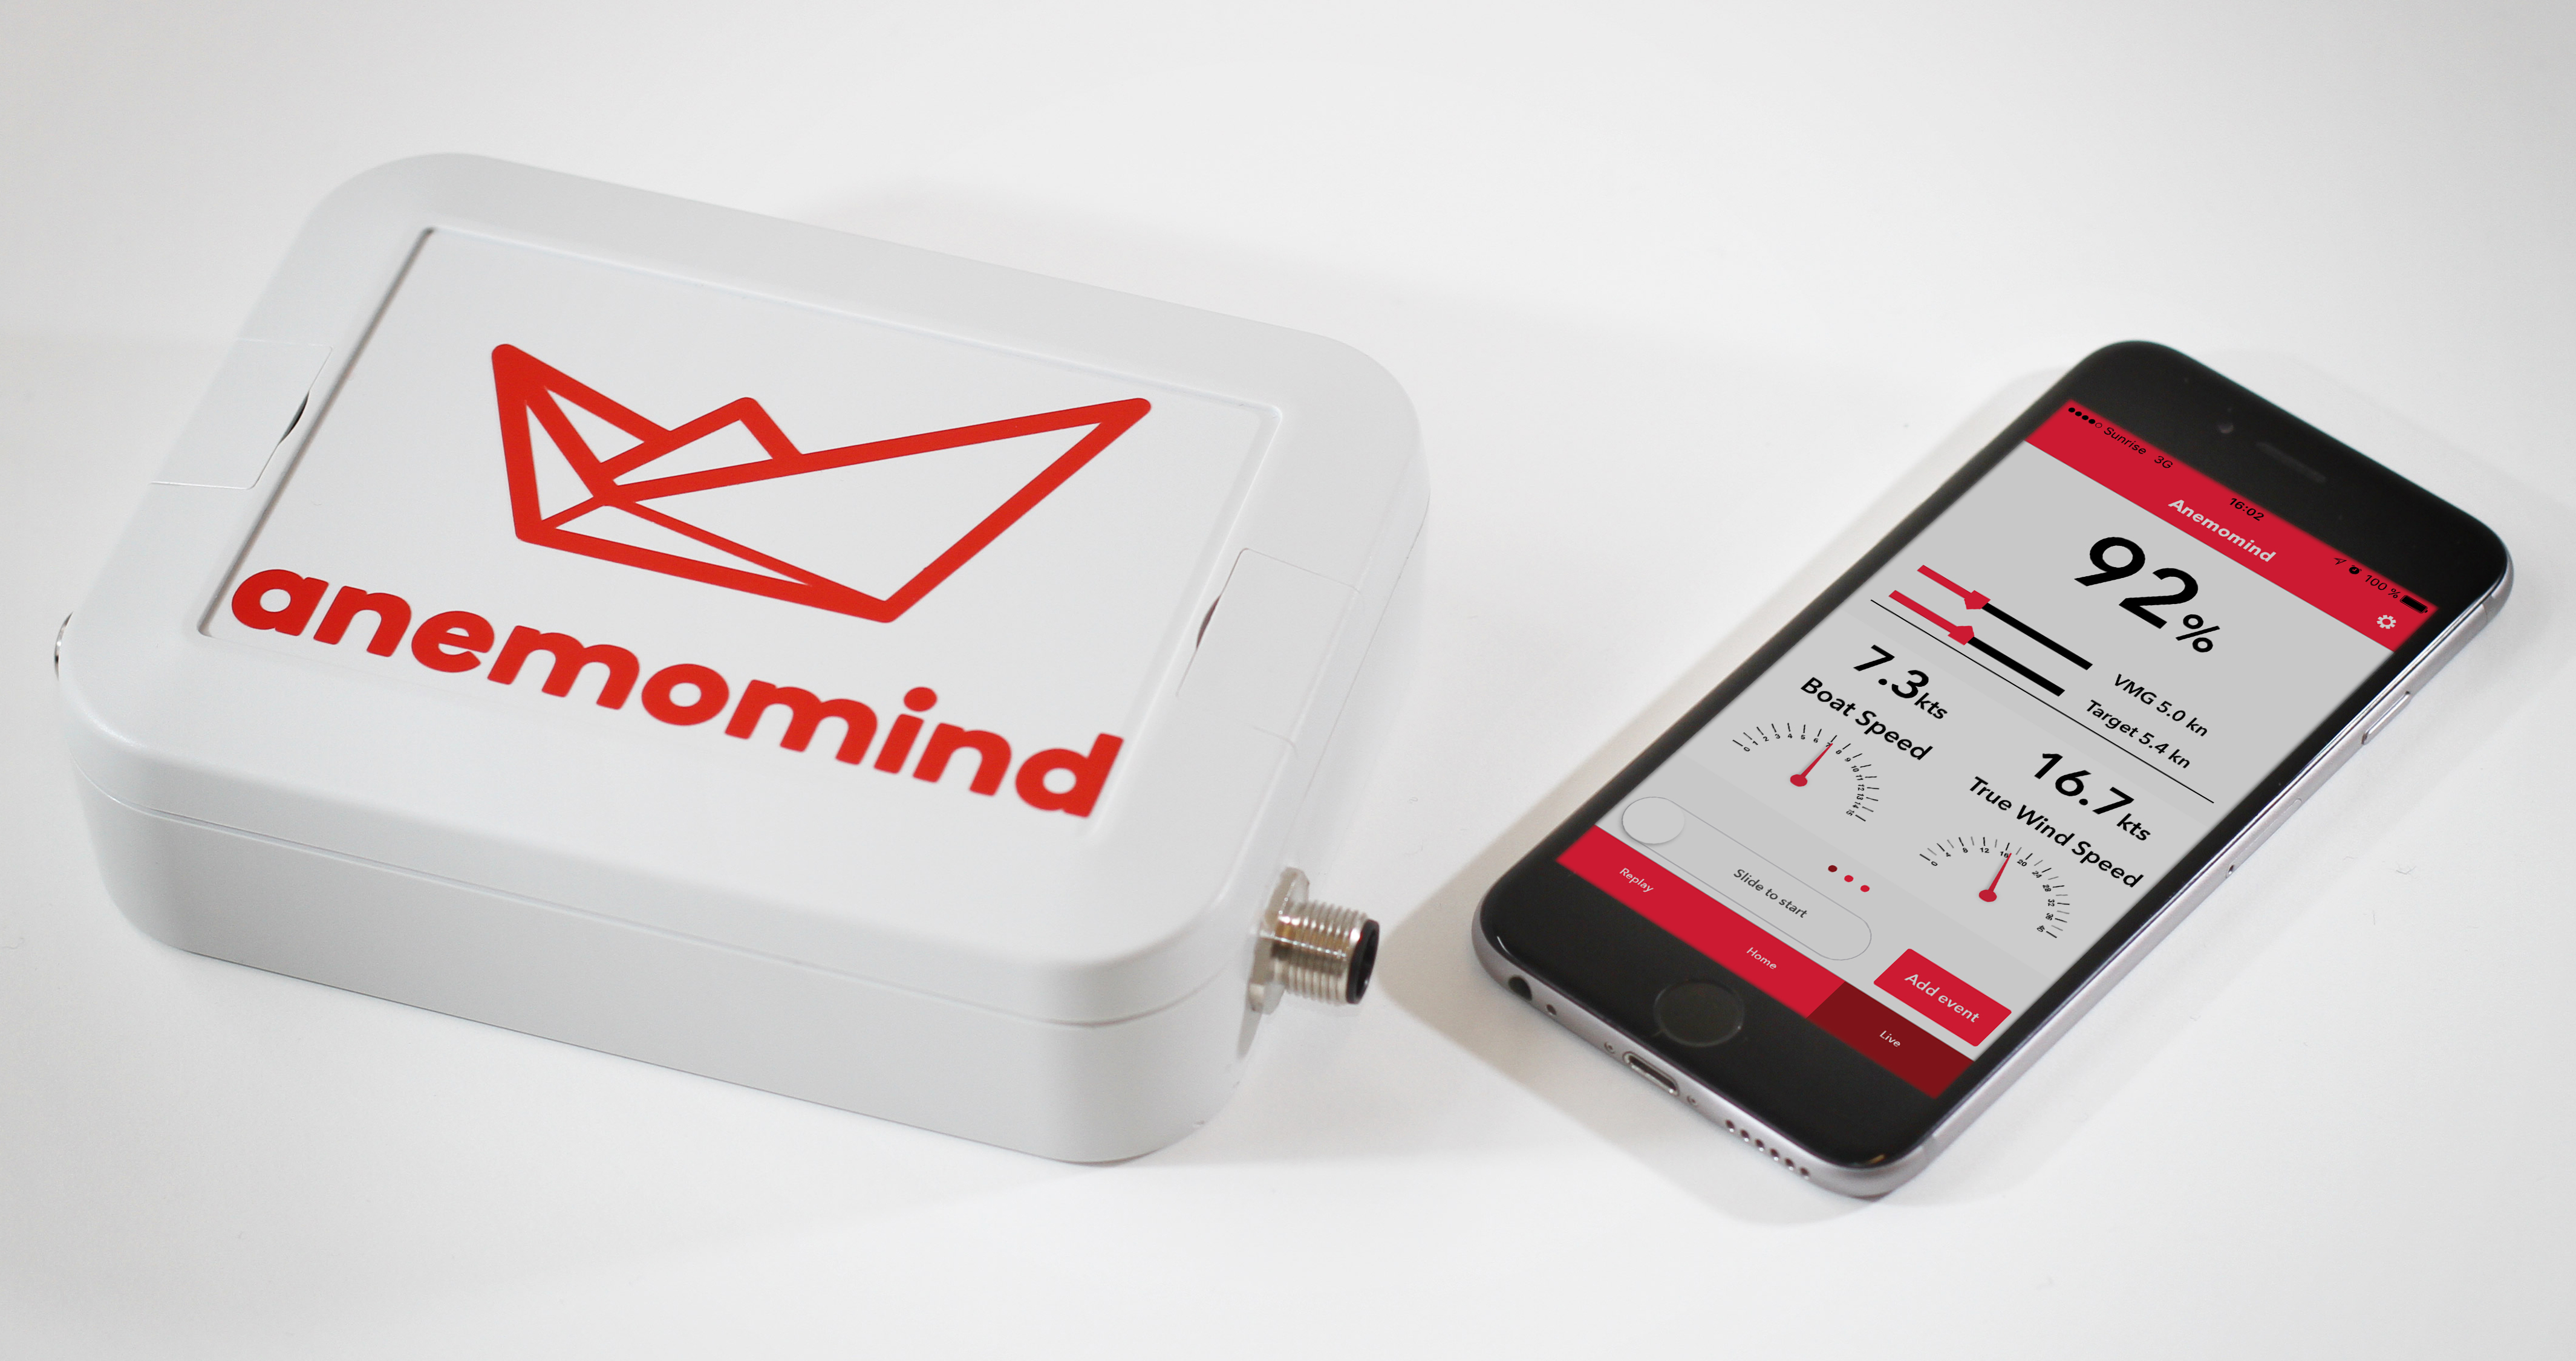
\includegraphics[width=\the\colwidth]{../images/anemobox10.jpg}
  \subheader{What you get}
  You can either buy or rent the Anemobox. The full package includes
  \begin{itemize}
    \item The Anemobox
    \item One year subscription to Anemolab
    \item iOS application for synchronization and real-time display
    \item An iPad
  \end{itemize}
  
  
  \textbf{TODO}
  Pricing information.
  Discounts?
  Predefined packages? (e.g. [rent anemobox+ipad][rent anemobox][buy anemobox]


  \subheader{Minimum requirements}
  To use the Anemobox, you need at least
  \begin{itemize}
    \setlength\itemsep{-0.1cm}
    \item A boat equipped with an NMEA2000/NMEA0183 wind sensor
    \item An iOS device, such as iPad or iPhone
    \item 9-24 Volts DC power supply
  \end{itemize}
  In addition, the Anemobox can receive data from other NMEA connected sensors too, such as magnetic compass or water speed.
}
\anemoparagraph{\the\haligniii}{\the\valignii}{
  \subheader{Feature summary}
  %% \begin{itemize}
  %%   \setlength\itemsep{-0.1cm}
  %% \end{itemize}

  {  
    \scriptsize
    \featuretable{
      Auto calibrated true wind computation & Boat performance computation \\
      Wireless connectivity Bluetooth 4.0 and WiFi & Data logging with automatic cloud sync \\
      Waterproof & NMEA 0183 and 2000 input/output \\
      10Hz satellite positioning (GPS, GLONASS and BeiDou) & Cloud-based sharing and visualization platform at www.anemolab.com \\
    }
  }
  \subheader{Specs}
  {
    \scriptsize
    \spectable{Embedded sensors}{
      GPS networks & multi-GNSS (GPS/QZSS, GLONASS and BeiDou) \\
      GPS accuracy & 2.5 m CEP \\
      GPS Frequency & 1-10 Hz \\
      External GPS support & NMEA 0183 and 2000 \\
      Inertial Measurement Unit &	9 axis, 1kHz \\
      Compass & 3 axis magnetometer, compensated with 3 gyroscopes \\
    }
    \spectable{Processing Characteristics}{
      Processing & dual-core, dual-threaded Intel® Atom CPU at 500 MHz \\
      RAM & 1GB \\
      Logging storage & 8GB \\
      System storage & 4GB \\
    }
    \spectable{Connections}{
      Wireless & Wifi, Bluetooth 4.0 \\
      8-poles IP67 connector & Power, NMEA input + output \\
      NMEA 2000 connector & Power, data input + output \\
    }
    \spectable{Physical Characteristics}{
      Size & 11 $\times$ 15 $\times$ 4 cm \\
      Weight & 227 g \\
    }
    \spectable{Electrical Characteristics}{
      Supply voltage & 9--24 V DC \\
      Power consumption & 1.5 W \\
      Current at 12V & 0.12 A \\
    }
  }
}



%% Lydia thought that the Order Form should be an a separate sheet,
%% so that the client can keep this information sheet. I think that
%% is a good idea.
\iffalse
  \mainheader{\the\haligni}{\the\valigniii}{Order Form}
  \anemoparagraph{\the\haligni}{\the\valigniv}{
    \subheader{Order specification}

    Please fill the number of items you want to buy in the left column.

    \medskip
    \rowcolors{2}{white}{white}
    \begin{tabularx}{\colwidth}{|l|X|r|}
      \hline 
      Quantity & Description & Price \\ \hline
      & Buy anemobox & CHF 2000 \\ \hline
      & Rent anemobox for 1 year & CHF 300 \\ \hline
    \end{tabularx}
  }

  \anemoparagraph{\the\haligniii}{\the\valigniv}{
    \subheader{Contact information}
    \textfield{First name}
    \textfield{Family name}
    \textfield{Street address}
    \textfield{Zip-code}
    \textfield{City}
    \textfield{Country}
    \textfield{E-mail address}
    \textfield{Phone}
  }
\fi
\end{tikzpicture}
\end{document} 

